%%
%% Academic journal article (Elsevier elsarticle).
%% Template from Overleaf gallery: Academic journal
%%   https://www.overleaf.com/latex/templates/tagged/academic-journal
%% Compile on Overleaf: pdfLaTeX, main.tex
%% Upload screenshots/ together with this file.
%%
\documentclass[preprint,12pt]{elsarticle}

\usepackage[T1]{fontenc}
\usepackage[utf8]{inputenc}
\usepackage[english]{babel}
\usepackage{amsmath,amssymb}
\usepackage{booktabs}
\usepackage{tabularx}
\usepackage{graphicx}
\usepackage{hyperref}
\usepackage{url}
\usepackage{tikz}
\usetikzlibrary{arrows.meta,positioning,fit,calc}

\graphicspath{{screenshots/}{../legal_multiagent/}}

\journal{ITMO University Practice Report}

\begin{document}
\begin{frontmatter}

\title{A multi-agent system for parsing court acts\\
and retrieving analogous practice from Russian courts of general jurisdiction}

\author{A.~Senichenkova}
\affiliation{organization={ITMO University},
            addressline={Kronverkskiy pr., 49},
            city={Saint Petersburg},
            postcode={197101},
            country={Russia}}

\begin{abstract}
We present a multi-agent assistant for case cards and judgment texts from Russian courts of general jurisdiction (SOY). The task is not outcome classification. A card is normalized into a structured Case~Graph; comparable practice is retrieved from an index; a draft position may cite only case IDs that exist in that index. Orchestration uses LangGraph: a linear graph of eleven nodes and six playbooks; nodes outside the plan are skipped. The act-split corpus ($\approx 1.86$ million rows) is loaded into SQLite. Without an LLM key the system relies on rules and index statistics; a large language model is optional. On 30 automated tests we observe correct query routing, article-and-region precision@5 of at least $60\,\%$, and Guard rejection of citations whose identifiers are missing from the index.
\end{abstract}

\begin{keyword}
multi-agent systems \sep judicial practice \sep information retrieval \sep LangGraph \sep Case Graph \sep courts of general jurisdiction
\end{keyword}

\end{frontmatter}

\begin{highlights}
\item Normalization of an SOY card and act splits into a single Case~Graph.
\item A linear agent graph with a playbook plan instead of a rigid pipeline.
\item Analog retrieval by article, region, judge, and fabula-token overlap.
\item Guard accepts citations only if the identifiers exist in the SQLite index.
\item The system is not an outcome classifier and is not legal advice.
\end{highlights}

\section{Introduction}

Open collections of SOY judgments are large, mixed, and poorly suited to manual search for ``similar cases.'' A case card stores metadata and sometimes the HTML of the act; a parallel corpus stores the act split into a header, the facts (fabula), and the operative part. There is no gold outcome label, case kinds are mixed, and wording of articles and results is not standardized.

Legal-AI setups often reduce to predicting a sentence or a charge~\cite{zhong2020legal,chalkidis2022lexglue}. A practising lawyer needs a different loop: see what is already known about the case, find comparable practice, and sketch a position---without treating corpus statistics as a court forecast. Large language models readily invent citations~\cite{magesh2024hallucination}, so generation must stay tied to the corpus.

This paper describes \texttt{legal\_multiagent}. The contributions are as follows.

\begin{enumerate}
\item A target case representation---Case~Graph---and ETL from two sources (JSONL cards and parquet act-splits).
\item A linear multi-agent graph on LangGraph~\cite{langgraph2024} with six playbooks and explicit skipping of unused nodes.
\item Analog search over a SQLite index and a hybrid score, not over unconstrained model text.
\item A Guard: a draft is accepted only if every cited identifier exists in the index.
\item Explicit limits: the system does not classify outcomes and is not legal advice.
\end{enumerate}

\section{Related work}

\textbf{Legal NLP.} Benchmarks such as LexGLUE~\cite{chalkidis2022lexglue} and LEGAL-BERT~\cite{chalkidis2020legalbert} measure classification, entity extraction, and NLI on English law. Surveys of legal AI~\cite{zhong2020legal} treat outcome prediction as a central task---a framing we deliberately avoid: our corpus has no reliable label, and a ``conviction probability'' would create false confidence~\cite{lockey2021trust}.

\textbf{Case retrieval.} COLIEE~\cite{rabelo2022coliee} and models such as BERT-PLI~\cite{shao2020bertpli} treat case retrieval as ranking precedents. We address the same user need on Russian SOY acts, but with rules and lexical overlap and without fine-tuning an encoder, so the score stays explainable and the index is easy to reproduce.

\textbf{RAG and legal LLMs.} Retrieval-augmented generation~\cite{lewis2020rag} and applied legal models~\cite{cui2023survey} mix retrieved fragments into the answer. Our Respond node builds markdown only from fields of the shared state; free generation, when enabled, is limited to act reading and wording.

\textbf{Multi-agent systems.} The classical view~\cite{wooldridge2009mas} separates roles and protocols. For LLM agents, conversational stacks such as AutoGen~\cite{wu2023autogen} are common. LangGraph~\cite{langgraph2024} gives an explicit state graph, which is more convenient than a prompt chain when some nodes must stay silent depending on the scenario.

\section{Data and task}

\subsection{Sources}

We use two corpora that agents never scan as raw files.

\begin{itemize}
\item \texttt{docs.json} --- JSONL SOY cards: metadata, case movement, and sometimes the HTML of the act.
\item \texttt{correct\_df\_splitted\_text.parquet} --- act splits: \texttt{text\_1} (header), \texttt{text\_2} (fabula), \texttt{text\_3} (operative part). After all 200 parts are loaded, the index holds $1{,}862{,}811$ cases.
\end{itemize}

Table~\ref{tab:kinds} shows the mix of the full parquet index by case kind. The corpus is civil: 138 criminal records. That limits use on criminal practice and is why the system is not framed as a ``sentence predictor.''

\begin{table}[t]
\centering
\caption{Composition of the full index after parquet ingest}
\label{tab:kinds}
\begin{tabular}{lr}
\toprule
Case kind & Records \\
\midrule
Civil & $1{,}609{,}786$ \\
Administrative & $161{,}766$ \\
Unknown & $91{,}121$ \\
Criminal & $138$ \\
\midrule
Total & $1{,}862{,}811$ \\
\bottomrule
\end{tabular}
\end{table}

\subsection{Task}

The input is a lawyer's query and optional \texttt{case\_id} / case number. The output is markdown: a dossier, a timeline, qualification, an analog table, a risk note, appeal remarks, and a draft position. Requirements:

\begin{enumerate}
\item do not predict the outcome of the proceeding;
\item do not cite cases that are absent from the index;
\item run without a language model if no API key is set.
\end{enumerate}

\section{Method}

\subsection{Case Graph}
\label{sec:casegraph}

A card and a parquet row are mapped to one Pydantic schema: identifier, number, court, judge, region, instance, case kind, charges/claim articles, event timeline, fabula, operative part, card outcome and act outcome, and gaps. Articles are extracted with regular expressions from card fields and from the concatenated act text. For parquet rows, case kind and instance are inferred from the header (for example, ``ugolovn\ldots\ delo'', civil numbers of the form $2$-, appellate numbers of the form $33$-).

\subsection{Index}

Normalized graphs are written to SQLite (\texttt{case\_store.sqlite}). Analog search does not scan raw JSONL or parquet. Ingest supports sources \texttt{parquet}, \texttt{docs}, and \texttt{both}, a row limit, and a database reset. Already stored parquet IDs are not overwritten; a later parquet pass fills missing fields on a card that was ingested first. The full corpus was loaded with batch inserts and WAL.

\subsection{Analog score}

Candidates are selected by article number (with a fallback text filter if exact matches are few) and ranked by the additive score
\begin{equation}
s = 5\cdot\mathbb{I}_{\mathrm{art}} + 3\cdot\mathbb{I}_{\mathrm{judge}} + 2\cdot\mathbb{I}_{\mathrm{reg}} + 1.5\cdot\mathbb{I}_{\mathrm{inst}} + \mathrm{Jaccard}(q, f),
\end{equation}
where the indicators are matches on article, judge, federal subject, and instance, and $\mathrm{Jaccard}$ is the share of shared tokens of length $\ge 3$ between the query/fabula $q$ and the candidate fabula hint $f$ after stop-word removal. The score is then normalized by the maximum in the result list. The weights deliberately make the article stronger than the judge; lexical overlap can still promote a different article, which is why the test threshold for article precision@5 is $60\,\%$, not $80\,\%$.

\subsection{Agent graph}

The shared state is \texttt{AgentState}: query, playbook, plan, card, analogs, intermediate reports, \texttt{final\_answer}, \texttt{steps\_done}, \texttt{gaps}. The graph is linear (Fig.~\ref{fig:graph}). The Orchestrator picks a playbook by query rules (appeal, draft, risk, analogs, dossier) and, if a key is set, may revise the choice through an LLM. An explicit \texttt{--playbook} is never overridden by the model. A node runs only if its name is in \texttt{plan}; otherwise the log records \texttt{name:skip}.

\begin{figure}[t]
\centering
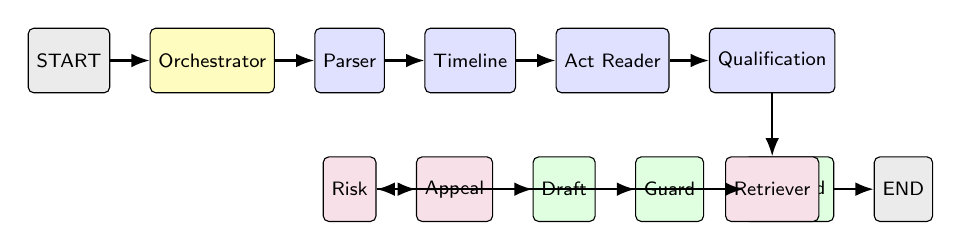
\begin{tikzpicture}[
  font=\scriptsize\sffamily,
  box/.style={draw, rounded corners=2pt, align=center, inner sep=3pt, minimum height=8.2mm},
  arr/.style={-{Latex}, thick}
]
\node[box, fill=black!8] (st) {START};
\node[box, fill=yellow!25, right=5mm of st] (or) {Orchestrator};
\node[box, fill=blue!12, right=5mm of or] (pa) {Parser};
\node[box, fill=blue!12, right=5mm of pa] (ti) {Timeline};
\node[box, fill=blue!12, right=5mm of ti] (ac) {Act Reader};
\node[box, fill=blue!12, right=5mm of ac] (qu) {Qualification};
\node[box, fill=purple!12, below=8mm of pa] (ri) {Risk};
\node[box, fill=purple!12, right=5mm of ri] (ap) {Appeal};
\node[box, fill=green!12, right=5mm of ap] (dr) {Draft};
\node[box, fill=green!12, right=5mm of dr] (gu) {Guard};
\node[box, fill=green!12, right=5mm of gu] (re) {Respond};
\node[box, fill=black!8, right=5mm of re] (en) {END};
\node[box, fill=purple!12] (rt) at (qu |- ri) {Retriever};
\draw[arr] (st) -- (or);
\draw[arr] (or) -- (pa);
\draw[arr] (pa) -- (ti);
\draw[arr] (ti) -- (ac);
\draw[arr] (ac) -- (qu);
\draw[arr] (qu) -- (rt);
\draw[arr] (rt) -- (ri);
\draw[arr] (ri) -- (ap);
\draw[arr] (ap) -- (dr);
\draw[arr] (dr) -- (gu);
\draw[arr] (gu) -- (re);
\draw[arr] (re) -- (en);
\end{tikzpicture}
\caption{Linear graph of \texttt{legal\_multiagent}. Yellow: routing. Blue: card and act parsing. Purple: practice and assessment. Green: draft and answer. Nodes outside \texttt{plan} are skipped.}
\label{fig:graph}
\end{figure}

Node roles:

\begin{description}
\item[Parser] loads a Case~Graph from the index by id or case number.
\item[Timeline] compresses the movement log.
\item[Act Reader] extracts fabula and operative part from splits or HTML; with an LLM key it may deepen the parse.
\item[Qualification] reconciles articles on the card and in the act.
\item[Retriever] ranks analogs by the score above.
\item[Risk] summarizes outcome frequencies among analogs and states that this is not a court forecast.
\item[Appeal] comments on the typical appellate fate of the act given the retrieved practice.
\item[Drafting] writes a draft that may cite only IDs present in state.
\item[Guard] checks cited IDs against the index.
\item[Respond] prints markdown only from filled state fields.
\end{description}

Six playbooks select node subsets (Table~\ref{tab:playbooks}).

\begin{table}[t]
\centering
\caption{Playbooks and nodes that run}
\label{tab:playbooks}
\begin{tabularx}{\linewidth}{lX}
\toprule
Playbook & Plan \\
\midrule
\texttt{dossier} & parser, timeline, act\_reader, qualification, respond \\
\texttt{analogs} & parser, qualification, retriever, respond \\
\texttt{risk} & parser $\ldots$ retriever, risk, guard, respond \\
\texttt{appeal} & parser $\ldots$ retriever, appeal, draft, guard, respond \\
\texttt{draft} & parser, act\_reader, qualification, retriever, draft, guard, respond \\
\texttt{full} & the full chain \\
\bottomrule
\end{tabularx}
\end{table}

\subsection{Optional language model}

The module \texttt{llm.py} calls an OpenAI-compatible endpoint (by default Ollama Cloud, model \texttt{gpt-oss:20b}). If \texttt{OLLAMA\_API\_KEY} is empty, \texttt{invoke\_text} / \texttt{invoke\_json} return \texttt{None} and nodes stay on heuristics. This keeps a reproducible offline path separate from a paid or networked path.

\section{Implementation}

The package targets Python~3.11+ with \texttt{langgraph}, \texttt{pydantic}, \texttt{pyarrow}, and \texttt{streamlit}. Entry points:

\begin{itemize}
\item CLI: \texttt{python -m legal\_multiagent ingest|status|ask};
\item library: \texttt{run\_agent(query, case\_id, case\_number, playbook)};
\item UI: \texttt{streamlit run legal\_multiagent/ui.py} --- index status, ingest, query, analog table, session history.
\end{itemize}

All three interfaces reuse the same \texttt{ingest}, \texttt{CaseStore}, and \texttt{run\_agent}. The full index is about $69$~GB; \texttt{--limit 3000} is enough for development.

Figures~\ref{fig:ui-query}--\ref{fig:ui-steps} show a live run of the Streamlit UI against the full index. The query is a Russian request to find similar tax-arrears cases; the playbook is set to \texttt{analogs}. The index reports $1{,}862{,}811$ cases (Fig.~\ref{fig:ui-query}). The answer lists twenty ranked analogs with article, outcome, judge, and score (Fig.~\ref{fig:ui-results}). Unused nodes are skipped: the step log is \texttt{orchestrator:analogs} $\to$ \texttt{parser:skip} $\to$ $\ldots$ $\to$ \texttt{qualification} $\to$ \texttt{retriever} $\to$ $\ldots$ $\to$ \texttt{respond} (Fig.~\ref{fig:ui-steps}).

\begin{figure}[t]
\centering
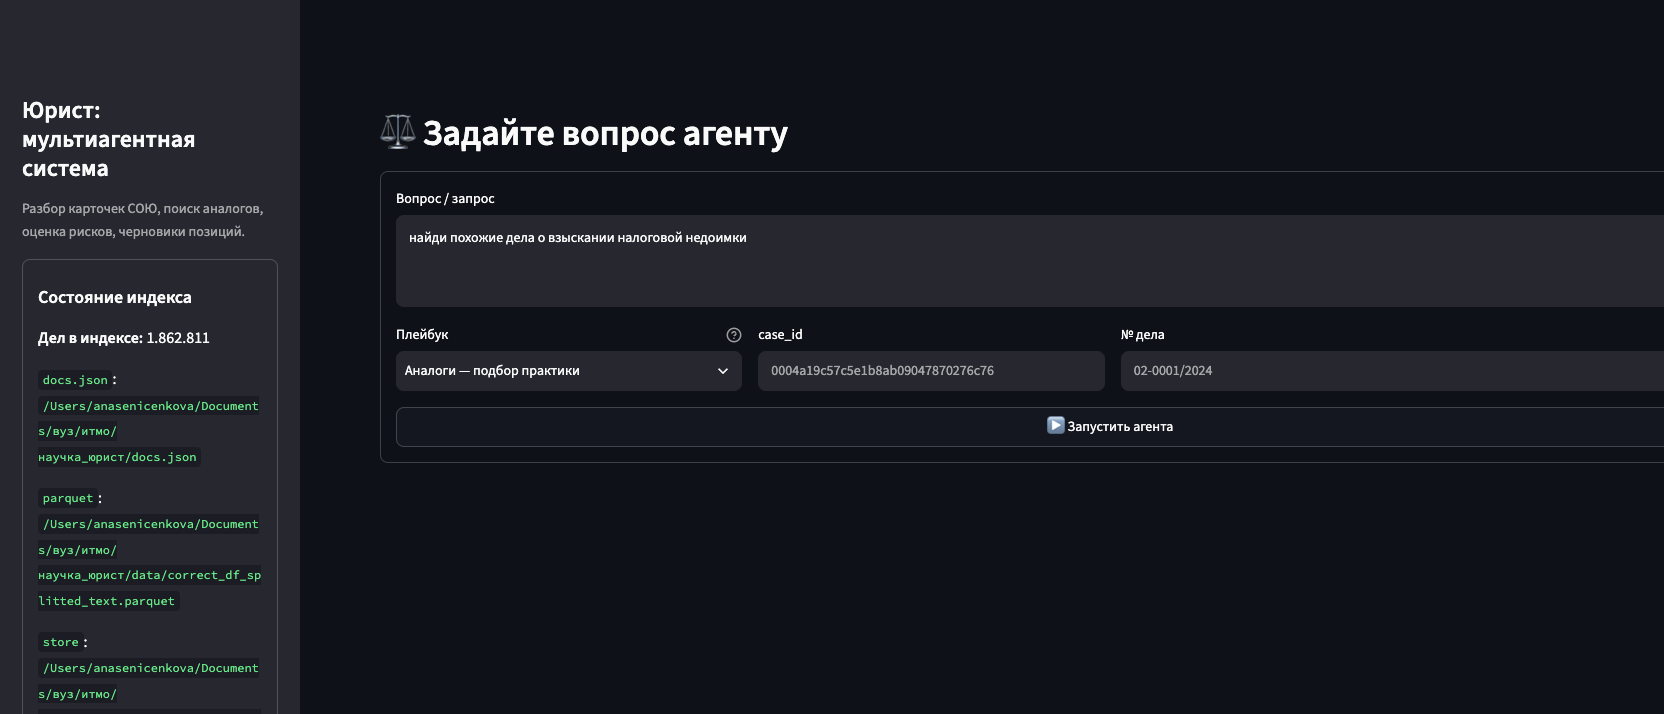
\includegraphics[width=\linewidth]{01_ui_query_crop.png}
\caption{Streamlit query form. Sidebar: $1{,}862{,}811$ cases in SQLite. Main pane: query ``find similar cases on recovery of tax arrears'' and playbook \texttt{analogs}.}
\label{fig:ui-query}
\end{figure}

\begin{figure}[t]
\centering
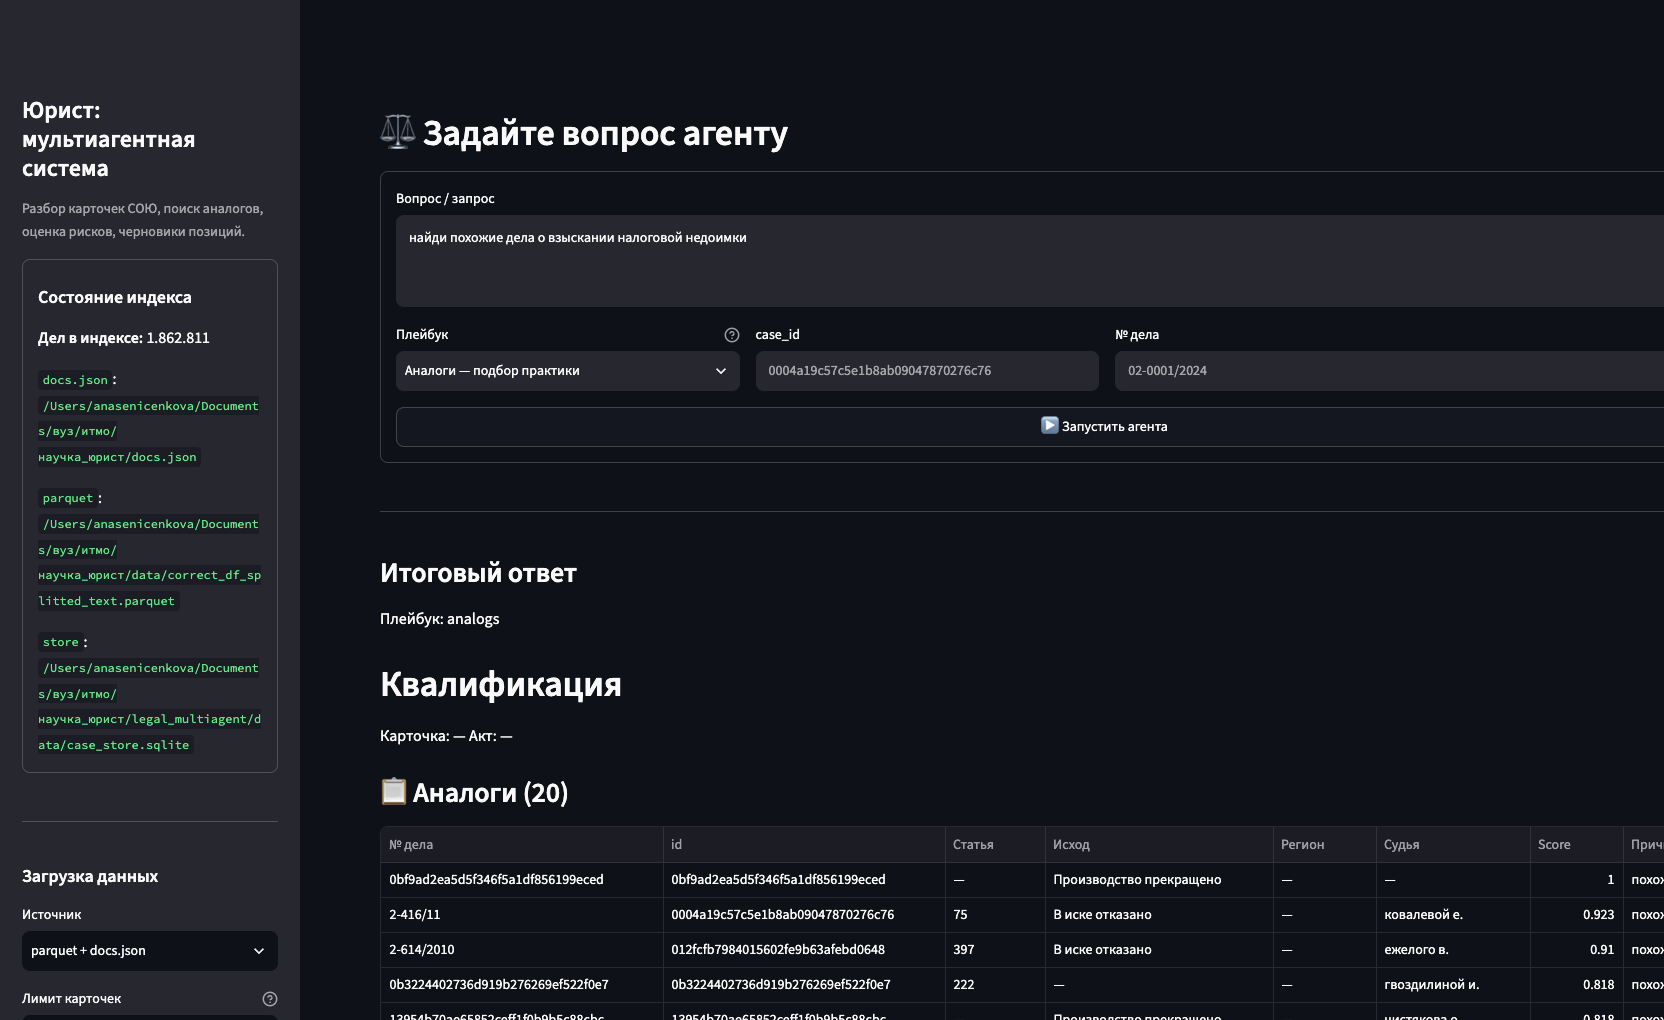
\includegraphics[width=\linewidth]{02_ui_results.png}
\caption{Agent answer after playbook \texttt{analogs}: qualification block and a table of 20 analogs (case number, id, article, outcome, region, judge, score).}
\label{fig:ui-results}
\end{figure}

\begin{figure}[t]
\centering
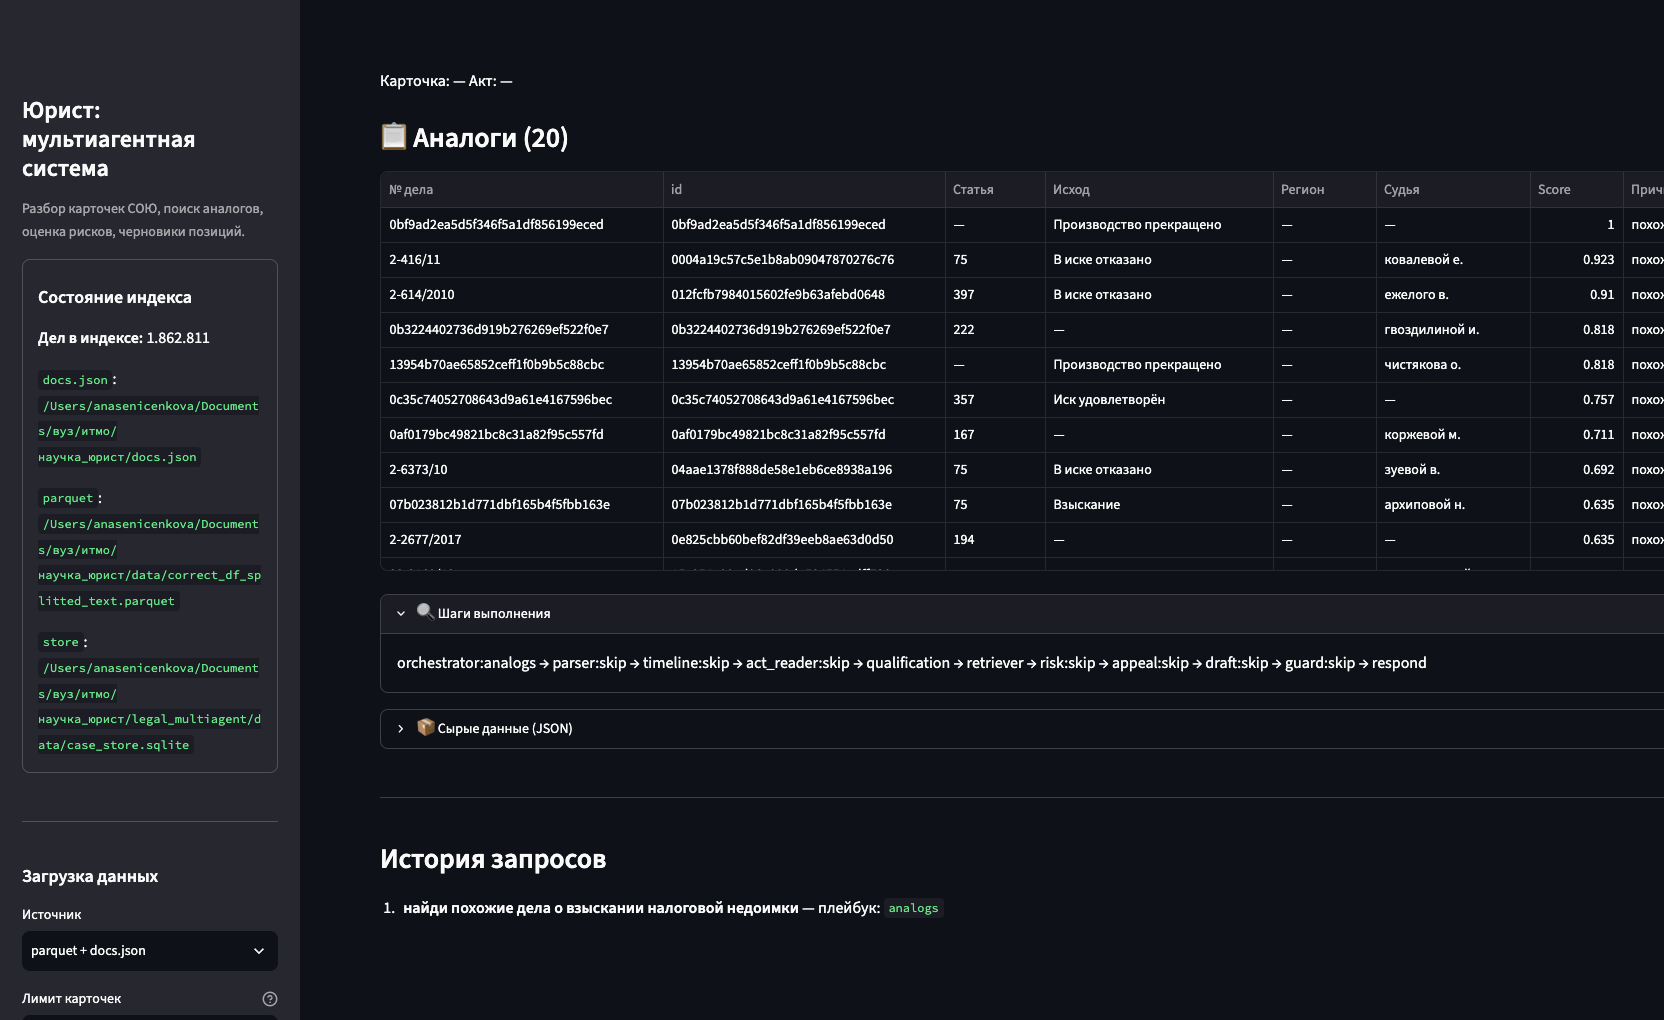
\includegraphics[width=\linewidth]{03_ui_steps.png}
\caption{The same run with the execution-step expander open. Nodes outside the playbook plan are marked \texttt{skip}; Retriever and Respond run.}
\label{fig:ui-steps}
\end{figure}

\section{Experiments}

Evaluation uses regression and qualitative automated tests (26~August 2026, Python~3.11.5), without calling an external LLM.

\subsection{Normalization and index}

Fifteen package tests (\texttt{test\_normalize}, \texttt{test\_system}) cover article parsing, Case~Graph assembly from a card and from parquet, score normalization, an empty hit list, the analog table, and ingest failure when files are missing. All 15 tests passed ($\approx 0.9$~s). Loading ten parquet rows into an isolated database yields exactly ten records.

\subsection{Agent quality}

Fifteen quality tests plus system tests: five query types route to the intended playbook; Parser finds and misses a card; Timeline counts events; Qualification catches an article mismatch; Act Reader reads splits; Retriever keeps at least $60\,\%$ of the top-5 with the same article and region; Respond adds no facts outside state; Guard rejects a citation of a missing id; Risk warns when the analog set is thin. All 30 available tests passed. An end-to-end \texttt{dossier} graph run is marked slow and requires LangGraph to be installed.

The UI screenshots in Figs.~\ref{fig:ui-query}--\ref{fig:ui-steps} are a qualitative check on the full index, not part of the automated suite: the playbook, skip chain, and analog table match the CLI verbose log for the same query.

\subsection{What was not measured}

LLM branches of Act~Reader / Risk / Appeal / Drafting were not run (no key in the test environment), nor were Streamlit clicks in CI. There is no lawyer-labeled ``this analog is useful'' set on the full corpus: lexical precision@5 is a proxy, not a measure of legal closeness.

\section{Discussion and limitations}

The system closes the gap between a raw act corpus and the working loop ``dossier --- practice --- draft'' without promising an outcome. The main limits follow from the data and the method.

\begin{enumerate}
\item The index is almost entirely civil; 138 criminal cases out of $1.86$ million.
\item Ranking is lexical: a matching article does not imply a similar fabula, and Jaccard can promote noise.
\item Without a key the wording is templated; with a key, hallucination risk appears. Guard covers identifiers, not the meaning of a norm.
\item Full SQLite needs tens of gigabytes and is not meant to be copied into git.
\end{enumerate}

Practical takeaway: the index and playbooks are useful as a practice-search assistant, not as a substitute for a human reading the act.

\section{Conclusion}

We described a multi-agent system that parses SOY case cards and retrieves analogous practice. A case is mapped to a Case~Graph, practice is searched in SQLite, the answer is assembled from graph state, and Guard blocks citations of missing cases. Automated tests show stable routing, retrieval, and the anti-hallucination check on identifiers. Next steps are fabula embeddings, lawyer relevance labels, LLM mocks for end-to-end tests, and precision/recall on a slice of the full index.

\section*{Acknowledgements}

This work was carried out as scientific practice at ITMO University. The system is not legal advice.

\bibliographystyle{elsarticle-num}
\bibliography{references}

\end{document}
